%%%%%%%%%%%%%%%%%%%%%%%%%%%%%%%%%%%%%%%%%
%
% Adapted by  Alvaro Gomariz (alvarogomarizc@gmail.com)
%from Claud D. Park (posquit0.bj@gmail.com) 

% Important note:
% This template must be compiled with XeLaTeX, the below lines will ensure this
%!TEX TS-program = xelatex
%!TEX encoding = UTF-8 Unicode
%
%%%%%%%%%%%%%%%%%%%%%%%%%%%%%%%%%https://www.overleaf.com/project/5d51b022da08c678a02b54b7%%%%%%%%

%----------------------------------------------------------------------------------------
%	PACKAGES AND OTHER DOCUMENT CONFIGURATIONS
%----------------------------------------------------------------------------------------

\documentclass[12pt, a4paper]{ag-cv} % A4 paper size by default, use 'letterpaper' for US letter
% \documentclass[12pt, a4paper]{ag-cv} % A4 paper size by default, use 'letterpaper' for US letter


\newcommand{\cvtype}{long} % short or long
\newcommand{\awardsmoney}{no} % yes or no
\newcommand{\showsupervisors}{no} % yes or no
\newcommand{\authornames}{long} % short or long
\newcommand{\publicationstype}{long} % short or long

% \ifthenelse{\equal{\cvtype}{short}}
%     { %short
%     \geometry{left=1.5cm, top=1.5cm, right=1.5cm, bottom=1.5cm, footskip=.5cm}
%     }
%     {%long
%     \geometry{left=2.5cm, top=2.5cm, right=2.5cm, bottom=2.5cm, footskip=.5cm}
%     % \geometry{left=2.4cm, top=2.5cm, right=2.4cm, bottom=2.5cm, footskip=.5cm}
%     }

\geometry{left=2.5cm, top=2.5cm, right=2.5cm, bottom=2.5cm, footskip=.5cm}
% \geometry{left=2.8cm, top=2.5cm, right=2.8cm, bottom=2.5cm, footskip=.5cm}

    

\usepackage{multicol}
\usepackage{parallel}

\usepackage{pdfpages}


% \ifthenelse{\equal{\cvtype}{short}}
%     {\geometry{left=1.5cm, top=1.5cm, right=1.5cm, bottom=2cm, footskip=.5cm} }
%     {\geometry{left=1.9cm, top=1.5cm, right=1.9cm, bottom=2cm, footskip=.5cm}}
% \geometry{left=1.5cm, top=1.5cm, right=1.5cm, bottom=2cm, footskip=.5cm} % Configure page margins with geometry
% \geometry{left=2cm, top=1.5cm, right=2cm, bottom=2cm, footskip=.5cm}


\fontdir[fonts/] 

% Color for highlights
\definecolor{awesome}{HTML}{1c85c7} % Uncomment if you would like to specify your own color


\renewcommand{\acvHeaderSocialSep}{\quad\textbar\quad} % If you would like to change the social information separator from a pipe (|) to something else

%----------------------------------------------------------------------------------------
%	PERSONAL INFORMATION
%	Comment any of the lines below if they are not required
%----------------------------------------------------------------------------------------
 
\name{}{Alvaro Gomariz}
% \address{Imfeldstrasse 103, CH-8037 Z\"urich}

% \email{alvarogomarizc@gmail.com}
\email{alvaro.gomariz@roche.com}
\orcid{0000-0002-6172-5190}
\linkedin{alvarogomariz}
\gscholar{https://scholar.google.com/citations?hl=en&user=v4JtSZcAAAAJ}
\mobile{ +41 (0)76 773 14 72}

% \extrainfo{\href{https://scholar.google.com/citations?hl=en&user=v4JtSZcAAAAJ}{Google Scholar}}% Other text you want to include on this line

% Available options: circle|rectangle,edge/noedge,left/right
%  \photo[circle,noedge,right]{portrait}

% \position{Bioimage Analysis Researcher}
% \position{Computer Vi{\enskip\cdotp\enskip}Security Expert} % Your expertise/fields


% \quote{
% My passion is to build tools that enable a data-based understanding of life, for which I investigate synergies between machine learning, computer vision, and life sciences. 
% While I have focused on research in my 6 years of experience, I have also engaged in product management and development with the aim of making a positive impact in the world. 
% } % A quote or statement

\quote{
% VARIANT GROUP: summary-quote — pick one active paragraph; keep the rest commented.
% VARIANT quote-roche-cscoe — tailored to Roche imaging/clinical-AI scientist roles  [ACTIVE]
ML Scientist with over 10 years of experience in machine learning for biomedical imaging and healthcare, including a PhD in Computer Vision and 5+ years in the pharmaceutical industry. I focus on identifying and realizing high-impact opportunities for ML in healthcare, from research to clinical trials, and on translating cutting-edge methods into robust, rigorously evaluated solutions. I have led cross-disciplinary projects that turn complex imaging and multimodal data into evidence for decision-making.
% VARIANT quote-foundation — foundation-model-oriented (prior applications)  [INACTIVE]
% Lead ML Scientist with over 10 years of experience designing, training, and adapting deep learning models to solve complex clinical problems. With a PhD in Computer Vision and 5+ years in the pharmaceutical industry, I specialize in foundation models, multi-modality, and uncertainty estimation. I am highly focused on rigorous statistical evaluation, ensuring model robustness, and translating cutting-edge research into scalable, high-impact health applications.
% VARIANT quote-leadership — leadership/strategy-forward  [INACTIVE]
% Strategic machine learning (ML) leader with over 10 years of experience applying ML to solve complex clinical problems, including 5+ years in the pharmaceutical industry and 4+ years in technical leadership roles. I have led teams of 10+ scientists to deliver production-level ML software within highly regulated settings. I specialise in driving cross-disciplinary projects across diverse disease areas to translate cutting-edge research into scalable, high-impact AI solutions.
}

\makecvfooter{\today}{Alvaro Gomariz~~~·~~~Résumé}{\thepage} % Specify the letter footer with 3 arguments: (<left>, <center>, <right>), leave any of these blank if they are not needed

%----------------------------------------------------------------------------------------

\begin{document}

\makecvheader % Print the header

%----------------------------------------------------------------------------------------
%	CV/RESUME CONTENT
%	Each section is imported separately, open each file in turn to modify content
%----------------------------------------------------------------------------------------

%----------------------------------------------------------------------------------------
%	SECTION TITLE
%----------------------------------------------------------------------------------------

\cvsection{Experience}

%----------------------------------------------------------------------------------------
%	SECTION CONTENT
%----------------------------------------------------------------------------------------

\begin{cventries}

%------------------------------------------------

\cventryag
{Postdoctoral scientist} % Job title
{Roche} % Organization
{Switzerland} % Location
{Mar 2021 - Present} % Date(s)
{ % Description(s) of tasks/responsibilities
\begin{cvitems}
\item {Research on semi-supervised learning and domain adaptation for image segmentation in optical coherence tomography}
\item {Corporate software development practises for integration of scientific outcomes into product development}
\end{cvitems}
}

\cventryag
{Research assistant} % Job title
{ETH Zurich \& University Hospital Zurich} % Organization
{Switzerland} % Location
{Sept 2016 - Feb 2021} % Date(s)
{ % Description(s) of tasks/responsibilities
\begin{cvitems}
\item {Machine learning research to facilitate the analysis of 3D microscopy images}
\item {Research translation in collaboration with biologists, clinicians, and healthcare companies}
\item {Development of image analysis tools for biologists with no programming experience}
\item {Teaching of bioimage analysis and confocal microscopy}
\ifthenelse{\equal{\cvtype}{short}}
    {\item {Supervision of 4 Master Thesis and 2 Semester Project students}}
    {}
\item Reviewer: IEEE Transactions on Medical Imaging, and MICCAI - Brain Lesion workshop
\end{cvitems}
}


% \cventryag
% {Consulting / Project manager} % Job title
% {MicroscopeIT} % Organization
% {Poland \& U.S.A. (remote)} % Location
% {Mar 2018 - Mar 2019} % Date(s)
% { % Description(s) of tasks/responsibilities
% \begin{cvitems}
% \item {Coordination of computer vision team for use of artificial intelligence in a bioimage analysis project}
% \item {Communication with clients to translate their research needs into a product}
% \end{cvitems}
% }


% \cventryag
% {Research student} % Job title
% {ETH Zurich \& University Hospital Zurich} % Organization
% {Switzerland} % Location
% {Sept 2015 - Aug 2016} % Date(s)
% { % Description(s) of tasks/responsibilities
% \begin{cvitems}
% \item {Building a custom image analysis pipeline to gain insight in the mechanisms of blood production}
% \item {Integrating ideas from research teams from different disciplines}
% \end{cvitems}
% }

% \cventryag
% {Research student} % Job title
% {ETH Zurich} % Organization
% {Switzerland} % Location
% {Feb 2015 - Sept 2015} % Date(s)
% { % Description(s) of tasks/responsibilities
% \begin{cvitems}
% \item {Research on registration of MRI images to address problems with sliding boundaries between organs}
% \end{cvitems}
% }

\cventryag
{Entrepreneur project} % Job title
{eMaging} % Organization
{Spain} % Location
{Oct 2013 - Sept 2014} % Date(s)
{ % Description(s) of tasks/responsibilities
\begin{cvitems}
\item {Building a start-up based on the development of medical devices for mobile phones}
\end{cvitems}
}

\cventryag
{Intern} % Job title
{Sedecal} % Organization
{Spain} % Location
{Dec 2013 - May 2014} % Date(s)
{ % Description(s) of tasks/responsibilities
\begin{cvitems}
\item {Documentation, support and development of preclinical imaging devices}
\end{cvitems}
}

\cventryag
{Research student} % Job title
{University Carlos III of Madrid} % Organization
{Spain} % Location
{July 2013 - July 2014} % Date(s)
{ % Description(s) of tasks/responsibilities
\begin{cvitems}
\item {Developing a pipeline for resolution studies of optical tomography systems}
\end{cvitems}
}

\ifthenelse{\equal{\cvtype}{short}}
    {}
    {
    \cventryag
    {Intern} % Job title
    {Murcia University} % Organization
    {Spain} % Location
    {June 2012 - July 2012} % Date(s)
    { % Description(s) of tasks/responsibilities
    \begin{cvitems}
    \item {Production and calibration of electrodes used for physiological measurements in diabetes studies}
    \end{cvitems}
    }
    
    \cventryag
    {Intern} % Job title
    {Medical Imaging Laboratory, Hospital Gregorio Marañón} % Organization
    {Spain} % Location
    {July 2011 - July 2011} % Date(s)
    { % Description(s) of tasks/responsibilities
    \begin{cvitems}
    \item {Measurement of the magnetic fields for a prototype of PET/MRI device}
    \end{cvitems}
    }
    }

%------------------------------------------------

\end{cventries}
%----------------------------------------------------------------------------------------
%	SECTION TITLE
%----------------------------------------------------------------------------------------

\cvsection{Education}

%----------------------------------------------------------------------------------------
%	SECTION CONTENT
%----------------------------------------------------------------------------------------

\begin{cventries}

%------------------------------------------------

\cventryag
{Doctor of Science in Computer Vision} % Degree
{ETH Zurich}
{Switzerland}
{Oct 2016 - Feb 2021} % Date(s)
{ % Description(s) bullet points
\begin{cvitems}
\item {Thesis title: ``Quantitative Fluorescence Microscopy with Marker-Efficient and Uncertainty-Aware Segmentation and Detection Using Deep Learning"}
\item {Supervisor: Prof.\ Orcun Goksel. Co-examiners: Prof.\
 C\'esar Nombela-Arrieta and Prof.\ Carolina W\"ahlby}
\end{cvitems}
}

\cventryag
{MSc in Biomedical Engineering} % Degree
{ETH Zurich}
{Switzerland}
{Oct 2014 - Sep 2016} % Date(s)
{ % Description(s) bullet points
\begin{cvitems}
% \item {Specialisation in Bioimaging}
\item {1st of class: awarded Willi-Studer Prize}
\ifthenelse{\equal{\cvtype}{short}}
    {\item {Master thesis: ``Applying 3D quantitative microscopy to study global topography and cellular interactions in the bone marrow"}}
    {\item {Master thesis: ``Applying 3D quantitative microscopy to study global topography and cellular interactions in the bone marrow", supervised by Prof.\ Gábor Székely, Prof.\ César Nombela-Arrieta, Dr.\ Simon N{\o}rrelykke, Dr.\ Szymon Stoma, and Dr.\ Grégory Paul}}
\ifthenelse{\equal{\cvtype}{short}}
    {\item {Semester project: ``Investigation of image registration for sliding boundaries"}}
    {\item {Semester project: ``Investigation of image registration for sliding boundaries", supervised by Prof.\ Orcun Goksel and Dr.\ Christine Tanner}}
\end{cvitems}
}

\cventryag
{BSc in Biomedical Engineering} % Degree
{University Carlos III of Madrid}
{Spain}
{Oct 2010 - Sep 2014} % Date(s)
{ % Description(s) bullet points
\begin{cvitems}
\item {1st of class: awarded Extraordinary End of Studies Award}
\ifthenelse{\equal{\cvtype}{short}}
    {\item {Bachelor thesis: ``Resolution study of optical tomography systems in microscopy"}}
    {\item {Bachelor thesis: ``Resolution study of optical tomography systems in microscopy", supervised by Prof.\ Jorge Ripoll}}
\end{cvitems}
}
%------------------------------------------------

\end{cventries}
%----------------------------------------------------------------------------------------
%	SECTION TITLE
%----------------------------------------------------------------------------------------

\cvsection{Skills}

%----------------------------------------------------------------------------------------
%	SECTION CONTENT
%----------------------------------------------------------------------------------------

\begin{cvskills}

\cvskill
{Languages} % Category
{English (fluent), Spanish (native), German (basic)} % Skills

\cvskill
{Programming} % Category
{Python (expert), Matlab (expert), R (intermediate), bash (intermediate)} % Skills

\cvskill
{Machine Learning} % Category
{TensorFlow, Keras, scikit-learn} % Skills

\cvskill
{Image Processing} % Category
{scikit-image, ITK, OpenCV, ImageJ, CellProfiler, ilastik, Imaris} % Skills

\cvskill
{Other} % Category
{git, \LaTeX, Vim, Adobe Photoshop/Illustrator} % Skills



\end{cvskills}
% \cvsection{Extracurricular Activities}

\begin{cvrefs}

\cvreference
{Student Representative of the Bachelor's Degree}
%in Biomedical Engineering}
{Meetings and decisions regarding the degree (2012~-~2014)}
{}

\cvreference
{Volunteer Lifeguard for the Spanish Red Cross}
{Vigilance and rescue in summer, with life Guard and First Aid Certificates}
{}

\cvreference
{Hobbies}
{Mountain-biking, swimming, playing guitar, scuba diving, philosophy}
{}


\end{cvrefs}


% %----------------------------------------------------------------------------------------
%	SECTION TITLE
%----------------------------------------------------------------------------------------

\cvsection{Awards and Scholarships}

%----------------------------------------------------------------------------------------
%	SECTION CONTENT
%----------------------------------------------------------------------------------------

\begin{cvhonors}

\cvhonor
{EXCITE PhD Excellence Award} % Position
{for outstanding PhD thesis in the field of biomedical imaging} % Committee
{2021} % Date(s)
{2500 CHF}

\cvhonor
{Hasler Stiftung grant} % Position
{to fund PhD project for 1 year} % Committee
{2019} % Date(s)
{50000 CHF}

\cvhonor
{Award to the best presented project} % Position
{at the 17\textsuperscript{th} Day of Clinical Research at University Hospital of Zurich, in the category Regenerative Medicine and Advanced Technologies} % Committee
{2018} % Date(s)
{1000 CHF}

\cvhonor
{Willi Studer Prize} % Position
{conferred to the student who attained the highest overall grade in the MSc in Biomedical Engineering at ETH Zurich} % Committee
{2017} % Date(s)
{3000 CHF}

%------------------------------------------------

\cvhonor
{Postgraduate Scholarship}
{granted by Fundación Caja Madrid to undertake a Master's degree at ETH Zurich}
{2014} % Date(s)
{9600 CHF}


\cvhonor
{Extraordinary End of Studies Award} % Position
{conferred to the student who attained the highest overall grade in the BSc in Biomedical Engineering at University Carlos III of Madrid} % Committee
{2014} % Date(s)
{}

%------------------------------------------------

\cvhonor
{Bachelor thesis awarded with special distinction} % Position
{for the best thesis of the graduating class} % Committee
{2014} % Date(s)
{}

\cvhonor
{Finalist in the StartUp Programme competition: SAGE Award}
{to the entrepreneur project eMaging}
{2014} % Date(s)
{}

\cvhonor
{Excellence Award 2014}
{granted to the 20 students with best grades that year in the University Carlos III of Madrid}
{2014} % Date(s)
{1000 CHF}

\cvhonor
{Travel grant}
{for presenting a poster and assisting to EMIM 2014 in Belgium}
{2014} % Date(s)
{300 CHF}

\cvhonor
{Collaboration scholarship}
{for conducting research 
% with the Materials Science and Engineering department of the Charles III University of Madrid}
at the University Carlos III of Madrid}
{2013} % Date(s)
{2000 CHF}

\cvhonor
{Scholarship}
{for new students with best entry grades at University Carlos III of Madrid}
{2010} % Date(s)
{1000 CHF}

\cvhonor
{Scholarship}
{for graduating high school with distinction (top 5\%) at IES Ramón Arcas Meca, Spain}
{2010} % Date(s)
{1200 CHF}

\end{cvhonors}

\pagebreak
\begin{center}
  \textit{ \Large{\textbf{Additional information}}}
\end{center}
\bigskip

%----------------------------------------------------------------------------------------
%	SECTION TITLE
%----------------------------------------------------------------------------------------

\cvsection{Scientific Contributions}

%----------------------------------------------------------------------------------------
%	SECTION CONTENT
%----------------------------------------------------------------------------------------

\cvsubsection{Journal articles}

\begin{cvpublications}

\cvpublication
{long}
{
\ifthenelse{\equal{\authornames}{short}}
    {\textbf{Gomariz A}, et al.~,}
    {\textbf{Gomariz A}, Kikuchi Y, Li Y, Albrecht A, Maunz A, Ferrara D, Lu H, Goksel O,}
}
{Joint semi-supervised and contrastive learning enables domain generalization and multi-domain segmentation}
{Medical Image Analysis}
{103, p.103575}
{2025}
{10.1016/j.media.2025.103575}


\cvpublication
{long}
{
\ifthenelse{\equal{\authornames}{short}}
    {Yamada Y, et al.~,}
    {Yamada Y, Nguyen TT, Impellizzieri D, Mineura D, Shibuya R, \textbf{Gomariz A}, Haberecker M, Nilsson J, Nombela-Arrieta C, Jungraithmayr W, Boyman O}
}
{Biased IL-2 signals induce Foxp3-rich pulmonary lymphoid structures and facilitate long-term lung allograft acceptance in mice}
{Nature Communications}
{1383 (14)}
{2023}
{10.1038/s41467-023-36924-z}

\cvpublication
{long}
{
\ifthenelse{\equal{\authornames}{short}}
    {Vijaykumar A, et al.~,}
    {Vijaykumar A, Helbling PM, Thelen F, Fazio S, Mun Y, Pereira AL, Zielińska KA, Buschl P, Zerkatje T, Loosli K, Isringhausen S, Menze B, Nagasawa T, Roeder I, \textbf{Gomariz A}, Manz MG, Yokomizo T, Nombela-Arrieta C}
}
{Tissue-scale mapping reveals a central role of hepatoblasts in the regulation of fetal liver hematopoiesis and stem cell maintenance}
{Developmental Cell}
{61, 901-918.e4}
{2026}
{10.1016/j.devcel.2026.01.011}


\cvpublication
{long}
{
\ifthenelse{\equal{\authornames}{short}}
    {\textbf{Gomariz A}, et al.~,}
    {\textbf{Gomariz A}, Portenier T, Nombela-Arrieta C, Goksel O,}
}
{Probabilistic Spatial Analysis in Quantitative Microscopy with Uncertainty-Aware Cell Detection using Deep Bayesian Regression}
{Science Advances}
{8 (5)}
{2022}
{10.1126/sciadv.abi8295}

\cvpublication
{long}
{
\ifthenelse{\equal{\authornames}{short}}
    {\textbf{Gomariz A}, et al.~,}
    {\textbf{Gomariz A}, Portenier T, Helbling PM, Isringhausen S, Suessbier U, Nombela-Arrieta C, Goksel O,}
}
{Modality Attention and Sampling Enables Deep Learning with Heterogeneous Marker Combinations in Fluorescence Microscopy}
{Nature Machine Intelligence}
{p.\ 1-13}
{2021}
{10.1038/s42256-021-00379-y}

\cvpublication
{long}
{
\ifthenelse{\equal{\authornames}{short}}
    {Isringhausen S, et al.~,}
    {Isringhausen S, Mun Y, Kovtonyuk L, Krautler N, Suessbier U, \textbf{Gomariz A}, Spaltro G, Helbling PM, Wong HC, Nagasawa T, Manz MG, Oxenius A, Nombela-Arrieta C,}
}
{Chronic viral infections persistently alter marrow stroma and impair hematopoietic stem cell fitness
}
{Journal of Experimental Medicine}
{218 (12)}
{2021}
{10.1084/jem.20192070}

\cvpublication
{long}
{
\ifthenelse{\equal{\authornames}{short}}
    {Ghazi S, et al.~,}
    {Ghazi S, Bourgeois S, \textbf{Gomariz A}, Bugarski M, Haenni D, Martins JR, Nombela-Arrieta C, Wagner CA, Hall AM, Eilidh C,}
}
{Multiparametric imaging reveals that mitochondria rich intercalated cells in the kidney collecting duct have a very high glycolytic capacity}
{The FASEB journal}
{34 (6), pp.\ 8510–8525}
{2020}
{10.1096/fj.202000273R}


\cvpublication
{long}
{
\ifthenelse{\equal{\authornames}{short}}
    {\textbf{Gomariz A}, et al.~,}
    {\textbf{Gomariz A}, Isringhausen S, Helbling PM, and Nombela-Arrieta C,}
}
{Imaging and spatial analysis of hematopoietic stem cell niches}
{Annals of the New York Academy of Sciences}
% ALT-ITEM — abbreviated venue name
% {Ann. N. Y. Acad. Sci}
{1466(1):5-16}
{2019}
{10.1111/nyas.14184}

\cvpublication
{long}
{
\ifthenelse{\equal{\authornames}{short}}
    {Hess M, et al.~,}
    {Hess M, \textbf{Gomariz A}, Goksel O, Ewald CY,}
}
{In-vivo quantitative image analysis of age-related morphological changes of C. elegans neurons reveals a correlation between neurite bending and novel neurite outgrowths}
{eNeuro}
{6(4)}
{2019}
{10.1523/ENEURO.0014-19.2019}

\cvpublication 
{long}
{
\ifthenelse{\equal{\authornames}{short}}
    {Agarwal P, et al.~,}
    {Agarwal P, Isringhausen S, Li H, Paterson AJ, He J, \textbf{Gomariz A}, Nagasawa T, Nombela-Arrieta C, and Bhatia R,}
}
{Mesenchymal niche-specific expression of Cxcl12 controls quiescence of treatment-resistant leukemia stem cells}
{Cell Stem Cell}
{24 (5), 769–784.e6}
{2019}
{10.1016/j.stem.2019.02.018}

\cvpublication 
{long}
{
\ifthenelse{\equal{\authornames}{short}}
    {\textbf{Gomariz A}, et al.~,}
    {\textbf{Gomariz A}, Helbling PM, Isringhausen S, Suessbier U, Becker A, Boss A, Nagasawa T, Paul G, Goksel O, Székely G, Stoma S, N{\o}rrelykke SF, Manz MG, and Nombela-Arrieta C,}
}
{Quantitative spatial analysis of haematopoiesis- regulating stromal cells in the bone marrow microenvironment by 3D microscopy}
{Nature Communications}
{9 (1)}
% ALT-ITEM — abbreviated venue name
% {Nat. Commun.}
{2018}
{10.1038/s41467-018-04770-z}

\cvpublication 
{long}
{
\ifthenelse{\equal{\authornames}{short}}
    {Takizawa H, et al.~,}
    {Takizawa H, Fritsch K, Kovtonyuk LV, Saito Y, Yakkala C, Jacobs K, Ahuja AK, Lopes M, Hausmann A, Hardt WD, \textbf{Gomariz A}, Nombela-Arrieta C, and Manz MG,}
}
{Pathogen-Induced TLR4-TRIF Innate Immune Signaling in Hematopoietic Stem Cells Promotes Proliferation but Reduces Competitive Fitness}
{Cell Stem Cell}
{21 (2), 225–240.e5}
{2017}
{10.1016/j.stem.2017.06.013}

\end{cvpublications}

\pagebreak
\cvsubsection{Conference papers}
\begin{cvpublications}
\cvpublication
{long}
{
\ifthenelse{\equal{\authornames}{short}}
    {Blasco Fernandez P, et al.~,}
    {Blasco Fernandez P, Bossuyt P, Daperno M, Kopylov U, Bouhnik Y, Karmiris K, Benmansour F, Gutierrez Becker B, Fraessle S, Stimpel B, Levitte S, \textbf{Gomariz A}}
}
{Quantifying Inter-Rater Reliability of Mucosal Features in Ulcerative Colitis Endoscopy}
{Journal of Crohn's and Colitis}
{Volume 20, Issue Supplement\_1}
{2026}
{10.1093/ecco-jcc/jjaf231.052}

\cvpublication
{long}
{
\ifthenelse{\equal{\authornames}{short}}
    {Gomariz A, et al.~,}
    {\textbf{Gomariz A}, Gutierrez-Becker B, Girycki R, Szostak P, Stimpel B, Levitte S, Abbasi-Sureshjani S}
}
{Assessing the Impact of Biopsy Artifacts on AI-Based Endoscopic Scoring for Ulcerative Colitis}
{Journal of Crohn's and Colitis}
{Volume 20, Issue Supplement\_1}
{2026}
{10.1093/ecco-jcc/jjaf231.699}

\cvpublication
{long}
{
\ifthenelse{\equal{\authornames}{short}}
    {Albuquerque T, et al.~,}
    {Albuquerque T, Yuce A, Herrmann MD, and \textbf{Gomariz A},}
}
{Characterizing the Interpretability of Attention Maps in Digital Pathology}
{arXiv}
{}
{2024}
{10.48550/arXiv.2407.02484}

\cvpublication
{long}
{
\ifthenelse{\equal{\authornames}{short}}
    {Bredell G, et al.~,}
    {Bredell G, Fischer M, Szostak P, Abbasi-Sureshjani S, and \textbf{Gomariz A},}
}
{The Importance of Downstream Networks in Digital Pathology Foundation Models}
{International Workshop on Foundation Models for General Medical AI - MICCAI}
{pp.\ 10-19}
{2024}
{10.1007/978-3-031-73471-7\_2}


\cvpublication
{long}
{
\ifthenelse{\equal{\authornames}{short}}
    {Ibañez V, et al.~,}
    {Ibañez V, Szostak P, Wong Q, Korski K, Abbasi-Sureshjani S, and \textbf{Gomariz A},}
}
{Integrating multiscale topology in digital pathology with pyramidal graph convolutional networks}
{IEEE International Symposium on Biomedical Imaging (ISBI)}
{pp.\ 1-4}
{2024}
{10.1109/ISBI56570.2024.10635702}

\cvpublication
{long}
{
\ifthenelse{\equal{\authornames}{short}}
    {Kikuchi Y, et al.~,}
    {Kikuchi Y, \textbf{Gomariz A}, Li Y, Lu H, Albrecht A, Ferrara D,}
}
{Device adaptation of optical coherence tomography (OCT) retinal layer segmentation algorithm using unlabeled target data}
{Investigative Ophthalmology \& Visual Science, ARVO abstract}
{(2023)}
{}
{}


\cvpublication
{long}
{
\ifthenelse{\equal{\authornames}{short}}
    {\textbf{Gomariz A}, et al.~,}
    {\textbf{Gomariz A}, Lu H, Li Y, Albrecht A, Maunz A, Benmansour F, Valcarcel AM, Luu J, Ferrara D, Goksel O,}
}
{Unsupervised Domain Adaptation with Contrastive Learning for OCT Segmentation}
{International Conference on Medical image computing and computer-assisted intervention (MICCAI)}
{pp.\ 351-361}
{2022}
{10.1007/978-3-031-16452-1\_34}

\cvpublication
{long}
{
\ifthenelse{\equal{\authornames}{short}}
    {Li Y, et al.~,}
    {Li Y, Lu H, Albrecht T, Maunz A, Neubert A, Benmansour F, \textbf{Gomariz A}, Luu J, Ferrara D}
}
{Deep learning (DL) to segment retinal layer disruption on optical coherence tomography (OCT) in neovascular age-related macular degeneration (nAMD)}
{Investigative Ophthalmology \& Visual Science, ARVO abstract}
{(2022)}
{}
{}


\cvpublication
{long}
{
\ifthenelse{\equal{\authornames}{short}}
    {\textbf{Gomariz A}, et al.~,}
    {\textbf{Gomariz A}, Lu H, Li Y, Albrecht A, Maunz A, Benmansour F, Luu J, Goksel O, Ferrara D,}
}
{A unified deep learning approach for OCT segmentation from different devices and retinal diseases}
{Investigative Ophthalmology \& Visual Science, ARVO abstract}
{(2022)}
{}
{}

\cvpublication
{long}
{
\ifthenelse{\equal{\authornames}{short}}
    {\textbf{Gomariz A}, et al.~,}
    {\textbf{Gomariz A}, Egli R, Portenier T, Nombela-Arrieta C, and Goksel O,}
}
{Utilizing Uncertainty Estimation in Deep Learning Segmentation of Fluorescence Microscopy Images with Missing Markers}
{IEEE International Symposium on Biomedical Imaging (ISBI)}
{pp.\ 371-374}
% ALT-ITEM — abbreviated venue name
% {IEEE ISBI}
{2021}
{10.1109/ISBI48211.2021.9434158}

\cvpublication
{long}
{
\ifthenelse{\equal{\authornames}{short}}
    {\textbf{Gomariz A}, et al.~,}
    {\textbf{Gomariz A}, Li W, Ozkan E, Tanner C, and Goksel O,}
}
{Siamese Networks with Location Prior for Landmark Tracking in Liver Ultrasound Sequences}
{IEEE International Symposium on Biomedical Imaging (ISBI)}
{pp.\ 1757-1760}
% ALT-ITEM — abbreviated venue name
% {IEEE ISBI}
{2019}
{10.1109/ISBI.2019.8759382}

\cvpublication
{long}
{
\ifthenelse{\equal{\authornames}{short}}
    {Goksel O, et al.~,}
    {Goksel O, Vishnevsky V, \textbf{Gomariz A}, and Tanner C,}
}
{Imaging of Sliding Visceral Interfaces During Breathing}
{IEEE International Symposium on Biomedical Imaging (ISBI)}
{pp.\ 298-301}
% ALT-ITEM — abbreviated venue name
% {IEEE ISBI}
{2016}
{10.1109/ISBI.2016.7493268}

\end{cvpublications}

% OPTIONAL oral-presentations — "Oral presentations at conferences" subsection  [OFF]
% % \pagebreak
% \cvsubsection{Oral presentations at conferences}

% \begin{cvpublications}

% \cvpreprint
% {short}
% {\textbf{Gomariz A}, Helbling PM, Isringhausen S, Suessbier U, Goksel O, and Nombela-Arrieta C,}
% {A Convolutional Neural Network-Based Pipeline for the Characterization of Large Bone Marrow Images in 3D Microscopy}
% {Swiss Light-Sheet Microscopy Workshop, Zurich}
% {2019}


% % \cvpreprint
% % {short}
% % {\textbf{Gomariz A}, Helbling PM, Isringhausen S, Suessbier U, Manz MG, Goksel O, and Nombela-Arrieta C}
% % {Deep learning methods for image-based understanding of the bone marrow microenvironment}
% % {Scientific Retreat on Experimental Hematology and Oncology, University Hospital of Zurich, Bergün}
% % {2019}

% \cvpreprint
% {short}
% {\textbf{Gomariz A}, Helbling PM, Isringhausen S, Suessbier U, Goksel O, Manz MG, and Nombela-Arrieta C,}
% {Quantitative Characterization of Bone Marrow Stroma Using Deep Learning}
% {Day of Clinical Research, University Hospital of Zurich}
% {2018}



% \cvpreprint
% {short}
% {\textbf{Gomariz A}, Helbling PM, Isringhausen S, Suessbier U, Becker A, Boss A, Nagasawa T, Paul G, Goksel O, Székely G, Stoma S, N{\o}rrelykke SF, Manz MG, and Nombela-Arrieta C,}
% {Quantitative characterization of bone marrow stromal topography using deep convolutional neural networks}
% {Seeing is Believing – Imaging the Molecular Processes of Life, EMBL, Heidelberg}
% {2017}


% \cvpreprint
% {short}
% {\textbf{Gomariz A}, Helbling PM, Isringhausen S, Suessbier U, Paul G, Székely G, Stoma S, N{\o}rrelykke SF, and Nombela-Arrieta C,}
% {Applying 3D quantitative microscopy to study global topography and cellular interactions in the bone marrow}
% {Image-based Systems Biology, Jena}
% {2016}


% \end{cvpublications}


% OPTIONAL invited-talks — "Invited talks" subsection  [OFF]
% \cvsubsection{Invited talks}

% \begin{cvpublications}
% \cvtalk
% {short}
% {Quantitative Fluorescence Microscopy with Marker-Efficient and Uncertainty-Aware Segmentation and Detection Using Deep Learning}
% {Visual Information and Interaction Seminar, Uppsala University}
% {2021}

% \cvtalk
% {short}
% {Microscopy-based characterization of the bone marrow structure using deep learning and spatial statistics}
% {Joint Immunology Meeting, University of Zurich and ETH Zurich}
% {2020}

% \cvtalk
% {short}
% {Image-based characterization of deep tissue fluorescence microscopy using convolutional neural networks}
% {Institute of Molecular Health Sciences, ETH Zurich}
% {2019}

% \cvtalk
% {short}
% {Deep learning methods for image-based understanding of the bone marrow microenvironment}
% % {Roche Innovation Center, Basel}
% {Roche, Basel}
% {2019}

% \cvtalk
% {short}
% {Image-based characterization of the bone marrow stroma using convolutional neural networks and spatial statistics}
% {Center for Microscopy and Image Analysis, University of Zurich}
% {2018}

% \cvtalk
% {short}
% {Quantitative spatial analysis of bone marrow tissues using 3D microscopy and deep learning}
% {Joint Cancer Meeting, University of Zurich and ETH Zurich}
% {2018}

% \end{cvpublications}

% OPTIONAL poster-presentations — "Poster presentations at conferences" subsection  [OFF]
% \cvsubsection{Poster presentations at conferences}

% \begin{cvpublications}

% \cvpreprint
% {short}
% {\textbf{Gomariz A}, Lu H, Li Y, Albrecht T, and Goksel O,}
% {Deep learning with labeled and unlabeled optical coherence tomography images}
% {Academia meets Industry: Basel Biozentrum / Roche Innovation Symposium}
% {2021}

% \cvpreprint
% {short}
% {\textbf{Gomariz A}, Lu H, Li Y, Albrecht T, and Goksel O,}
% {Deep semi-supervised learning for image segmentation in
% multi-domain optical coherence tomography}
% {Basel Postdoc Network Meeting, Kandersteg}
% {2021}

% \cvpreprint
% {short}
% {\textbf{Gomariz A}, Helbling PM, Isringhausen S, Suessbier U, Goksel O, Manz MG, and Nombela-Arrieta C,}
% {A deep learning pipeline for spatial characterization of bone marrow stroma}
% {14th Charles Rodolphe Brupbacher Symposium, Zurich}
% {2019}


% \cvpreprint
% {short}
% {\textbf{Gomariz A}, Helbling PM, Isringhausen S, Suessbier U, Becker A, Boss A, Nagasawa T, Paul G, Goksel O, Székely G, Stoma S, N{\o}rrelykke SF, Manz MG, and Nombela-Arrieta C,}
% {Spatial Analysis of the Bone Marrow Stroma Using Deep Learning}
% {Swiss Oncology \& Hematology Congress, Zurich}
% {2018}


% \cvpreprint
% {short}
% {\textbf{Gomariz A}, Helbling PM, Isringhausen S, Suessbier U, Becker A, Boss A, Nagasawa T, Paul G, Goksel O, Székely G, Stoma S, N{\o}rrelykke SF, Manz MG, and Nombela-Arrieta C,}
% {Convolutional Neural Networks in 3D Microscopy: Spatial Analysis of the Bone Marrow Microenvironment}
% {2nd NEUBIAS Conference, Szeged}
% {2018}


% \cvpreprint
% {short}
% {\textbf{Gomariz A}, Helbling PM, Isringhausen S, Suessbier U, Becker A, Boss A, Nagasawa T, Paul G, Goksel O, Székely G, Stoma S, N{\o}rrelykke SF, Manz MG, and Nombela-Arrieta C,}
% {Multiscale image-based quantitative analysis of bone marrow stromal network topology reveals strict spatial constraints for hematopoietic-stromal cellular interactions}
% {4th Lymphoid Tissue Meeting, St. Gallen}
% {2017}


% \cvpreprint
% {short}
% {\textbf{Gomariz A}, Helbling PM, Isringhausen S, Suessbier U, Becker A, Boss A, Nagasawa T, Paul G, Goksel O, Székely G, Stoma S, N{\o}rrelykke SF, Manz MG, and Nombela-Arrieta C,}
% {Applying 3D quantitative microscopy to study global topography and cellular interactions in the bone marrow}
% {Charles Rodolphe Brupbacher Symposium, Zurich}
% {2017}


% \cvpreprint
% {short}
% {\textbf{Gomariz A}, Remacha E, Vizcaino G, Corral A, Paarman M, Zacharakis G, Vaquero JJ, Desco M, Moscoso M, and Ripoll J,}
% {Protocol for Establishing the Resolution in Laser Sheet Microscopes}
% {European Molecular Imaging Meeting, Leuven}
% {2014}


% \cvpreprint
% {short}
% {\textbf{Gomariz A}, Remacha E, Vizcaino G, Corral A, Paarman M, Vaquero JJ, Desco M, Moscoso M, Scheffold F, and Ripoll J,}
% {Resolution Comparison between Laser Sheet Microscopy and Optical Projection Tomography}
% {European Molecular Imaging Meeting, Leuven}
% {2014}


% \end{cvpublications}

% 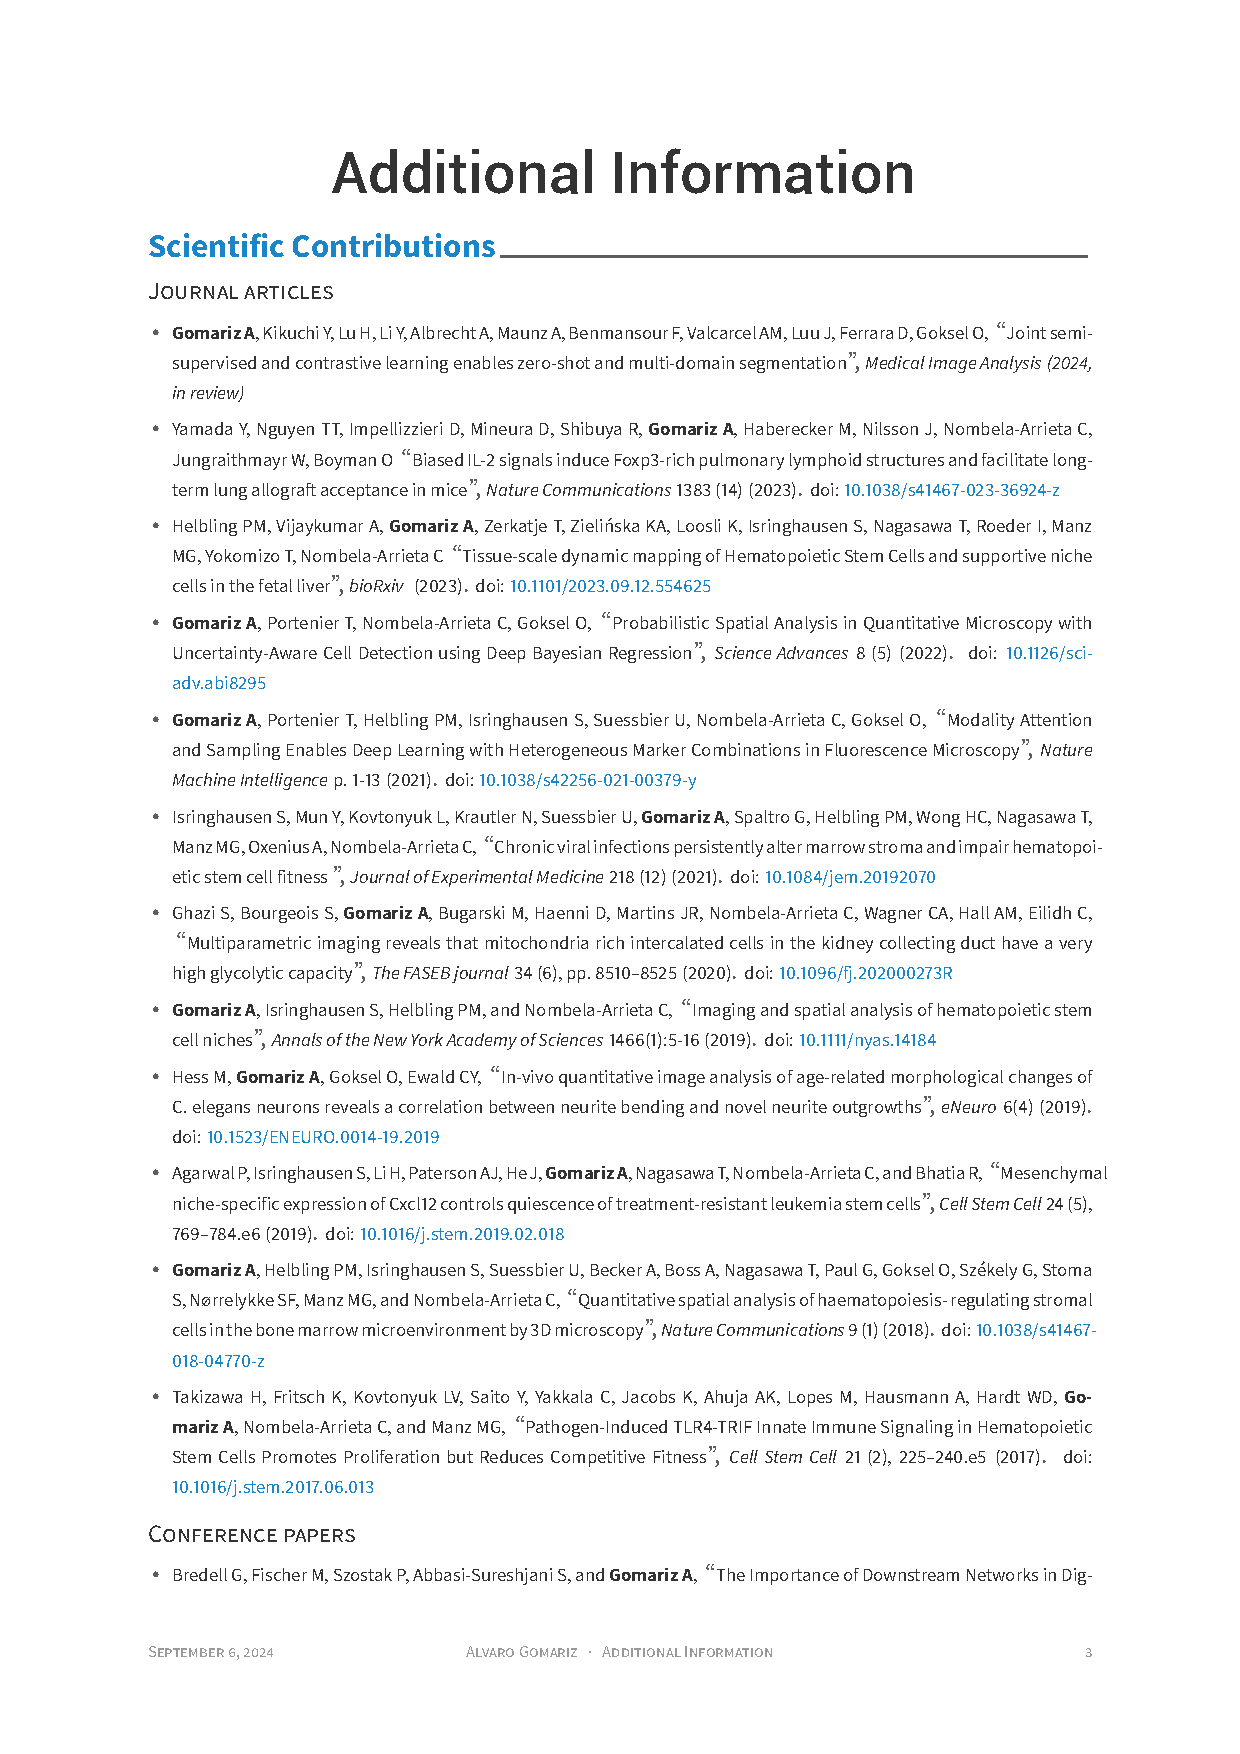
\includepdf[pages=-]{cv_additional.pdf}


% 
\cvsection{Student Supervision}

\begin{cvhonors}

\cvhonor
{Luca Widmer,}
{Master thesis: ``Versatile framework for application of deep learning in biological image analysis"
}
{2020}
{}

\cvhonor
{Raphael Egli,}
{Master thesis: ``Estimating segmentation uncertainty on fluorescence microscopy with heterogeneous modalities"
}
{2020}
{}

\cvhonor
{Efe Akmansu,}
{Master thesis: ``Cell detection on 3D fluorescence microscopy with CNNs"}
{2019}
{}

\cvhonor
{Kaan Akan,}
{Summer internship: ``Image analysis tool for applying CNNs on multidimensional images in biology"}
{2019}
{}

\cvhonor
{Grégoire Dauce,}
{Semester project: ``Suggestive annotation neural networks for bioimages"}
{2018}
{}

\cvhonor
{Weiye Li,}
{Semester project: ``Liver tracking in ultrasound sequences using neural networks"}
{2018}
{}

\cvhonor
{Max Hess,}
{Master thesis: ``Quantification of morphological changes in ageing C. elegans"}
{2017}
{}

\end{cvhonors}
% \cvsection{References}

\begin{cvrefs}

\cvreference
{Orcun Goksel}
{Professor at ETH Zurich}
{ogoksel@vision.ee.ethz.ch}

\cvreference
{César Nombela-Arrieta}
{Professor at the University of Zurich}
{Cesar.NombelaArrieta@usz.ch}

\cvreference
{Szymon Stoma}
{CEO of MicroscopeIT}
{szymon.stoma@ethz.ch}

\cvreference
{Simon F. Noerrelykke}
{Head of Image and Data Analysis Unit, ScopeM, ETH Zurich}
{simon.noerrelykke@scopem.ethz.ch}


\end{cvrefs}

% \let\thefootnote\relax\footnotetext{Scientific contributions are included in a supplementary document}


%----------------------------------------------------------------------------------------

\end{document}